%%%% FIGURE SHOWING GENOMUS ENCODED GENOTYPES CODING FROM GERMINAL VECTOR

\documentclass{standalone}% For the example only, any class will do

\usepackage{tikz}
\usetikzlibrary{arrows, automata, positioning}
\usetikzlibrary{shapes.geometric}

\begin{document}
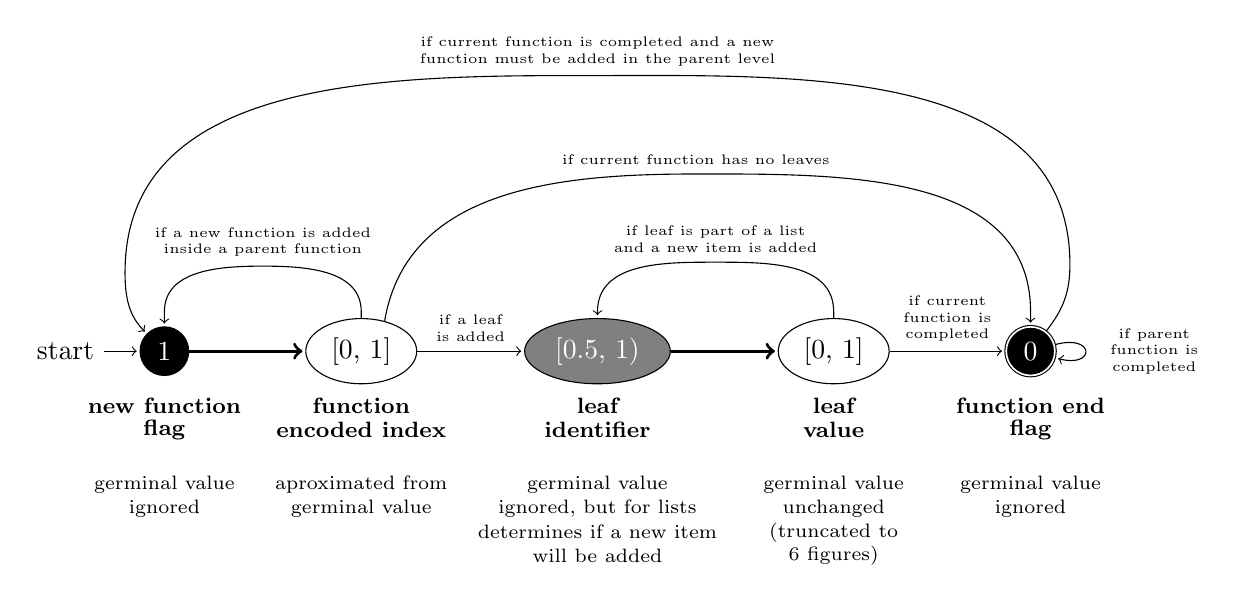
\begin{tikzpicture}[shorten >=1pt, node distance=2cm, auto]

% \draw[help lines] (0,0) grid (12,5);

% STATES
\node[initial, circle, fill=black, draw=black, text=white] (newF) at (0,1.7) {1};
\node[ellipse, fill=none, draw=black, text=black] (funcEncIdx) at (2.5,1.7) {[0, 1]};
\node[ellipse, fill=gray, draw=black, text=white] (leafId) at (5.5,1.7) {[0.5, 1)};
\node[ellipse, fill=none, draw=black, text=black] (leafValue) at (8.5,1.7) {[0, 1]};
\node[accepting, circle, fill=black, draw=black, text=white] (funcEnd) at (11,1.7) {0};

% COMMENTS TO STATES
\node[text width=2.2cm, text badly centered, font=\bfseries] at (0,1) {\footnotesize{new function}};
\node[text width=2.2cm, text badly centered, font=\bfseries] at (0,0.7) {\footnotesize{flag }};

\node[text width=2.2cm, text badly centered, font=\bfseries] at (2.5,1) {\footnotesize{function}};
\node[text width=2.2cm, text badly centered, font=\bfseries] at (2.5,0.7) {\footnotesize{encoded index}};

\node[text width=2.2cm, text badly centered, font=\bfseries] at (5.5,1) {\footnotesize{leaf}};
\node[text width=2.2cm, text badly centered, font=\bfseries] at (5.5,0.7) {\footnotesize{identifier}};

\node[text width=2.2cm, text badly centered, font=\bfseries] at (8.5,1) {\footnotesize{leaf}};
\node[text width=2.2cm, text badly centered, font=\bfseries] at (8.5,0.7) {\footnotesize{value}};

\node[text width=2.2cm, text badly centered, font=\bfseries] at (11,1) {\footnotesize{function end}};
\node[text width=2.2cm, text badly centered, font=\bfseries] at (11,0.7) {\footnotesize{flag }};

% COMMENTS ABOUT GERMINAL VALUES HANDLING
\node[text width=2.2cm, text badly centered] at (0,0) {\scriptsize{germinal value}};
\node[text width=2.2cm, text badly centered] at (0,-0.3) {\scriptsize{ignored}};

\node[text width=2.2cm, text badly centered] at (2.5,0) {\scriptsize{aproximated from}};
\node[text width=2.2cm, text badly centered] at (2.5,-0.3) {\scriptsize{germinal value }};

\node[text width=4.2cm, text badly centered] at (5.5,0) {\scriptsize{germinal value}};
\node[text width=4.2cm, text badly centered] at (5.5,-0.3) {\scriptsize{ignored, but for lists}};
\node[text width=4.2cm, text badly centered] at (5.5,-0.6) {\scriptsize{determines if a new item}};
\node[text width=4.2cm, text badly centered] at (5.5,-0.9) {\scriptsize{will be added}};

\node[text width=2.2cm, text badly centered] at (8.5,0) {\scriptsize{germinal value}};
\node[text width=2.2cm, text badly centered] at (8.5,-0.3) {\scriptsize{unchanged}};
\node[text width=2.2cm, text badly centered] at (8.5,-0.6) {\scriptsize{(truncated to}};
\node[text width=2.2cm, text badly centered] at (8.5,-0.9) {\scriptsize{6 figures)}};

\node[text width=2.2cm, text badly centered] at (11,0) {\scriptsize{germinal value}};
\node[text width=2.2cm, text badly centered] at (11,-0.3) {\scriptsize{ignored }};

% STRAIGHT ARROWS
\path[->, very thick] (newF) edge node {} (funcEncIdx);     
\path[->, font=\tiny, text width=1cm, text badly centered] (funcEncIdx) edge node {if a leaf is added} (leafId);
\path[->, very thick] (leafId) edge node {} (leafValue);
\path[->, font=\tiny, text width=1.5cm, text badly centered] (leafValue) edge node {if current function is completed} (funcEnd);
\path[->, font=\tiny, text width=1.5cm, text badly centered] (funcEnd) edge [loop right] node {if parent function is completed} (funcEnd);
 
% CURVED ARROWS
\draw[->, font=\tiny, text width=5.1cm, text badly centered] (funcEnd) to [out=52,in=-90] (11.5,2.8)
      to [out=90,in=0] (5.5,5.2) node[above,sloped] {if current function is completed and a new function must be added in the parent level} 
      to [out=180,in=90] (-0.5,2.7) 
      to [out=270,in=135] (newF);

\draw[->, font=\tiny, text width=2.6cm, text badly centered] (leafValue) to [out=90,in=-90] (8.5,2.2)
      to [out=90,in=0] (7,2.83) node[above,sloped] {if leaf is part of a list and a new item is added} 
      to [out=180,in=90] (5.5, 2.2) 
      to [out=270,in=90] (leafId);

\draw[->, font=\tiny, text width=4.3cm, text badly centered] (funcEncIdx) to [out=52.75,in=240] (2.8,2.1)
      to [out=80,in=180] (6.75,3.95) node[above,sloped] {if current function has no leaves} 
      to [out=0,in=90] (11, 2.2) 
      to [out=270,in=90] (funcEnd);
      
\draw[->, font=\tiny, text width=2.9cm, text badly centered] (funcEncIdx) to [out=90,in=-90] (2.5,2.2)
      to [out=90,in=0] (1.25,2.78) node[above,sloped] {if a new function is added inside a parent function} 
      to [out=180,in=90] (0, 2.2) 
      to [out=270,in=90] (newF);

\end{tikzpicture}
\end{document}